% !TEX TS-program = XeLaTeX
% use the following command:
% all document files must be coded in UTF-8
\documentclass[english]{textolivre}
% build HTML with: make4ht -e build.lua -c textolivre.cfg -x -u article "fn-in,svg,pic-align"

\journalname{Texto Livre}
\thevolume{15}
%\thenumber{1} % old template
\theyear{2022}
\receiveddate{\DTMdisplaydate{2022}{4}{28}{-1}} % YYYY MM DD
\accepteddate{\DTMdisplaydate{2022}{7}{18}{-1}}
\publisheddate{\DTMdisplaydate{2022}{8}{14}{-1}}
\corrauthor{Elih Sutisna Yanto}
\articledoi{10.35699/1983-3652.2022.39459}
%\articleid{NNNN} % if the article ID is not the last 5 numbers of its DOI, provide it using \articleid{} commmand 
% list of available sesscions in the journal: articles, dossier, reports, essays, reviews, interviews, editorial
\articlesessionname{articles}
\runningauthor{Yanto} 
%\editorname{Leonardo Araújo} % old template
\sectioneditorname{Daniervelin Pereira}
\layouteditorname{Leonado Araújo}

\title{Engaging pre-service English teachers in Sheltered Instruction Model – mediated content and language learning: a microethnographic classroom-based study}
\othertitle{Envolvendo professores de inglês pré-serviço em modelo de instrução protegido – conteúdo mediado e aprendizagem de línguas: um estudo microetnográfico baseado em sala de aula}
% if there is a third language title, add here:
%\othertitle{Artikelvorlage zur Einreichung beim Texto Livre Journal}

\author[1]{Elih Sutisna Yanto \orcid{0000-0003-0701-6454} \thanks{Email: \href{mailto:elih.sutisna@fkip.unsika.ac.id}{elih.sutisna@fkip.unsika.ac.id}}}
\affil[1]{Universitas Singaperbangsa Karawang, Faculty of Teachers Training and Education, Department of English Education, Karawang, West-Java, Indonesia.}

\addbibresource{article.bib}
% use biber instead of bibtex
% $ biber article

% used to create dummy text for the template file
\definecolor{dark-gray}{gray}{0.35} % color used to display dummy texts
\usepackage{lipsum}
\SetLipsumParListSurrounders{\colorlet{oldcolor}{.}\color{dark-gray}}{\color{oldcolor}}

% used here only to provide the XeLaTeX and BibTeX logos
\usepackage{hologo}

% if you use multirows in a table, include the multirow package
\usepackage{multirow}

% provides sidewaysfigure environment
\usepackage{rotating}

% CUSTOM EPIGRAPH - BEGIN 
%%% https://tex.stackexchange.com/questions/193178/specific-epigraph-style
\usepackage{epigraph}
\renewcommand\textflush{flushright}
\makeatletter
\newlength\epitextskip
\pretocmd{\@epitext}{\em}{}{}
\apptocmd{\@epitext}{\em}{}{}
\patchcmd{\epigraph}{\@epitext{#1}\\}{\@epitext{#1}\\[\epitextskip]}{}{}
\makeatother
\setlength\epigraphrule{0pt}
\setlength\epitextskip{0.5ex}
\setlength\epigraphwidth{.7\textwidth}
% CUSTOM EPIGRAPH - END

% LANGUAGE - BEGIN
% ARABIC
% for languages that use special fonts, you must provide the typeface that will be used
% \setotherlanguage{arabic}
% \newfontfamily\arabicfont[Script=Arabic]{Amiri}
% \newfontfamily\arabicfontsf[Script=Arabic]{Amiri}
% \newfontfamily\arabicfonttt[Script=Arabic]{Amiri}
%
% in the article, to add arabic text use: \textlang{arabic}{ ... }
%
% RUSSIAN
% for russian text we also need to define fonts with support for Cyrillic script
% \usepackage{fontspec}
% \setotherlanguage{russian}
% \newfontfamily\cyrillicfont{Times New Roman}
% \newfontfamily\cyrillicfontsf{Times New Roman}[Script=Cyrillic]
% \newfontfamily\cyrillicfonttt{Times New Roman}[Script=Cyrillic]
%
% in the text use \begin{russian} ... \end{russian}
% LANGUAGE - END

% EMOJIS - BEGIN
% to use emoticons in your manuscript
% https://stackoverflow.com/questions/190145/how-to-insert-emoticons-in-latex/57076064
% using font Symbola, which has full support
% the font may be downloaded at:
% https://dn-works.com/ufas/
% add to preamble:
% \newfontfamily\Symbola{Symbola}
% in the text use:
% {\Symbola }
% EMOJIS - END

% LABEL REFERENCE TO DESCRIPTIVE LIST - BEGIN
% reference itens in a descriptive list using their labels instead of numbers
% insert the code below in the preambule:
%\makeatletter
%\let\orgdescriptionlabel\descriptionlabel
%\renewcommand*{\descriptionlabel}[1]{%
%  \let\orglabel\label
%  \let\label\@gobble
%  \phantomsection
%  \edef\@currentlabel{#1\unskip}%
%  \let\label\orglabel
%  \orgdescriptionlabel{#1}%
%}
%\makeatother
%
% in your document, use as illustraded here:
%\begin{description}
%  \item[first\label{itm1}] this is only an example;
%  % ...  add more items
%\end{description}
% LABEL REFERENCE TO DESCRIPTIVE LIST - END


% add line numbers for submission
%\usepackage{lineno}
%\linenumbers

\begin{document}
\maketitle

\begin{polyabstract}
\begin{abstract}
This study employs the Sheltered Instruction (SI) model and a micro-ethnographic classroom-based study to develop the content (i.e., quantitative research in English Language Teaching) and language learning advancement of pre-service English teachers (henceforth PETS), which includes lesson planning and preparation, building a backdrop, comprehensible input, strategies, interaction, practice/application, lesson delivery, and assessment. Seventy English Education students enrolled in the Quantitative Research in English Language Teaching (ELT) course at Universitas Singaperbangsa Karawang, Indonesia, volunteered to take part in the study. In this study, data was gathered using students' work artifacts: questionnaires, in-class discussion notes, and reflective journals (daily notes). The findings of a qualitative study indicate the SI model of content and language learning helps PETS improve their academic language. This study also shows that employing SI as an intervention model could help pre-service English teachers improve their academic language skills in the content or subject area in the context of English as a foreign language.

\keywords{English language teaching \sep Quantitative research \sep Sheltered instruction model \sep Social cultural theory}
\end{abstract}

\begin{portuguese}
\begin{abstract}
Este estudo emprega o modelo Sheltered Instruction (SI) e um estudo microetnográfico baseado em sala de aula para desenvolver o conteúdo (ou seja, pesquisa quantitativa no ensino de inglês) e o avanço do aprendizado de idiomas de professores de inglês pré-serviço (doravante PETS), que inclui planejamento e preparação de aulas, construção de um pano de fundo, informações compreensíveis, estratégias, interação, prática/aplicação, apresentação de aulas e avaliação. Setenta estudantes de Educação Inglesa matriculados no curso de Pesquisa Quantitativa no Ensino da Língua Inglesa (ELT) na Universitas Singaperbangsa Karawang, da Indonésia, se ofereceram para participar do estudo. Neste estudo, os dados foram coletados usando artefatos de trabalho dos alunos: questionários, notas de discussão em sala de aula e diários reflexivos. Os resultados de um estudo de conteúdo qualitativo indicam que o modelo SI de conteúdo e aprendizagem de idiomas ajuda o PETS a melhorar sua linguagem acadêmica. Este estudo também mostra que empregar o SI como modelo de intervenção pode ajudar os professores de inglês em formação a melhorar suas habilidades de linguagem acadêmica no conteúdo ou área de assunto no contexto do inglês como língua estrangeira.

\keywords{Ensino de língua inglesa \sep Pesquisa quantitativa \sep Modelo de instrução protegido \sep Teoria sociocultural}
\end{abstract}
\end{portuguese}
% if there is another abstract, insert it here using the same scheme
\end{polyabstract}

\section{Introduction}\label{sec-intro}
In-service and pre-service teachers should be proficient in the range of subjects that they will be teaching to students. Apart from the variety of subjects, some studies indicate that discipline varies from one to another. Moreover, academic writings indicate the variety of one discipline compared to another. For this reason, teachers should be able to comprehend the disciplines both qualitatively and quantitatively. The corpus data information indicate that the disciplines are classified according to the topic area categories developed by Scopus, namely, life sciences, health sciences, physical sciences, social sciences, and humanities \cite{kwary_corpus_2019}. Social science areas such as action research have become widely attractive in education. However, the majority of textbooks on action research in education place a strong emphasis on qualitative research. Teachers and people who want to become teachers need to understand quantitative research if they want to be fully involved and do well in their careers. They must be able to interpret test scores (both in terms of how the test scores are derived and how the test scores are interpreted). It is also possible for them to make decisions based on data and be informed consumers of educational research, among other things.

The current study intends to document a micro-ethnographic, classroom-based study of PETS' participation in content and language learning, utilizing the Sheltered Instruction Observation Protocol (SIOP) methodology to improve pre-service teachers’ academic language skills (i.e., quantitative research in ELT). The students are in the English education major, but they are also required to take a course on Quantitative Research in English Language Research (henceforth QR in ELT). The Sheltered Instruction Observation Protocol (SIOP), which is based on research and has been proven to work, comes from the United States. This model is used for students in elementary and secondary schools learning English as a second language while also studying subjects like mathematics and science which are taught in English. The SIOP model, proposed by \textcite{echevarria_making_2017}, was used by the author in this study to engage PETS and to help PETS improve their academic language abilities, such as understanding, in a comprehensible manner, discipline-specific vocabulary, as well asproducing and interacting with  spoken and written texts typical in QR.

Researchers \cite{goldenberg_teaching_2008,moschkovich_using_2006,fatmawati_fractional_2019,farchan_analisis_2020,windarto_mathematical_2021} claim that mathematics is tightly linked to language and culture. In order for students of a foreign language to do well in mathematics, they must be very good at the language and know how to use it in a variety of situations \cite{kotsopoulos_mathematics_2007,morgan_language_2014,nacarato_role_2014,chen_research_2008}. Thus, in a content-based ELT classroom, students are not only learning English but also learning disciplines or content (i.e., QR in the ELT). Curriculum knowledge and English language skills must grow together in this content-based classroom \cite{gibbons_mediating_2003}. Additional empirical studies have demonstrated the importance of language in mathematics instruction \cite{barwell_heteroglossia_2012,goldenberg_teaching_2008}. Students' academic progress is greatly aided by the efforts of their content teachers (teachers who teach the subjects) \cite{gersten_lost_1999,reeves_secondary_2006}.

There are a lot of mathematics and statistics teachers who assume that students might have trouble understanding the language used in statistics \cite{bay-williams_is_2007,borgioli_equity_2008}. For example, the words "degree" and "table" have different meanings in everyday communication and in mathematics terminology. In daily communication, the words "degree" and "table" refer to graduation and a piece of furniture, respectively. In contrast, the terms "table" and "degree" in mathematics refer to an arrangement of numbers, symbols, or words displaying facts or relations, and the sum of the exponents for the variables in an algebraic expression. The students do not use these words in normal conversation \cite{kaplan_lexical_2009,lesser_english_2009,rubenstein_understanding_2002,watson_statistical_2006,winsor_bridging_2007}. As a result, the students do not know what they mean.

This article discusses how the SIOP model was implemented during the course of QR in ELT. Furthermore, this paper describes how this procedure unfolds for PETS enrolled in the QR in the ELT course, whether English is used as a foreign language (as a school topic) or as an additional language (as a means of communication). The application of the SIOP model in the context of pre-service English teachers remains unexplored. To address this gap, this article reports microethnographic classroom-based research using the SIOP model to advance PETS’ “content and language learning ability.” This involves lesson planning, background knowledge, understandable input, strategies, interaction, practice/application, and lesson presentation. Two research questions guide this investigation.

\begin{enumerate}
    \item How might the SIOP intervention model, help PETS enhance their academic language?
    \item How do PETS react to SIOP model activities and tasks?
\end{enumerate}

\section{Literature review}\label{sec-normas}
\subsection{The SIOP model's historical context}
The concept of "sheltered instruction," also known as "Specially Designed Academic Instruction in English" (SDAIE), refers to strategies used in the content area that are presented in English to students who do not speak English in order to help them understand the subject matter while also developing their English language skills at the same time \cite{hansen-thomas_sheltered_2008,crawford_impact_2008}. The goal was to address the language and educational needs of second-language immigrant and non-immigrant learners in schools in the United States of America, both in terms of language and education \cite{echevarria_making_2008,echevarria_siop_2010,hansen-thomas_sheltered_2008}. Shelter Instruction is made up of great teaching practices or instructional procedures that have been shown to be effective in the classroom.

\textcite{hansen-thomas_sheltered_2008} identified five criteria for Sheltered Instruction:

\begin{enumerate}
    \item Implementation of cooperative learning activities with appropriately designed diverse students;
    \item A strong emphasis on academic language as well as key content vocabulary;
    \item The intelligent use of English Language Learners' (ELL) first language as a comprehensibility-enhancing tool.
    \item The use of hands-on activities including authentic materials, lectures, and modeling, and
    \item Instruction and use of learning processes in a direct and explicit manner.
\end{enumerate}

This approach is supported by the theories of proximal development by \textcite{vygotskii_mind_1978} and multiple intelligence by \textcite{gardner_educational_1989}, and it is characterized by collaborative learning, peer tutoring, scaffolding, and other strategies to aid students in excelling at each stage and transitioning from one to the next.

\subsection{Sheltered Instruction Observation Protocol (SIOP)}\label{sec-conduta}
SIOP focuses on "the practice of integrating language development with strategies for making curricular content more understandable to English Language Learners" (ELLs) \cite[p. 334]{short_developing_2012}. Teachers who teach English as a second language (ESL) can use SIOP to show how to teach ESL students and how to improve their content and language literacy skills. Therefore, they can understand the content-area text. SIOP, according to \textcite{echevarria_using_2011}, provides teachers with a well-articulated practical instructional procedure. SIOP is equivalent to content-based instruction with bilingual programs (CBI), integrated content and language learning (CLIL), and language immersion programs. There are numerous advantages to SIOP, including the ability to improve academic performance, accelerate the development of academic English abilities, and use content-related language to scaffold meaning-making tasks \cite{murie_when_2001,song_content-based_2006}.

Based on \textcite{echevarria_making_2017}, SIOP embraces the following eight main components:

\begin{enumerate}
    \item Lesson Planning: Each SIOP session focuses on a distinct language and content objective that is tied to the curriculum and standards and delivered in a systematic manner. Teachers plan their lessons very carefully. They use relevant content concepts, extra materials, and content adaptation when necessary, as well as interesting activities that combine concepts and language practice (see Appendix \ref{appendix}).
    \item Establishing a Foundation: As part of their cognitive processes, teachers establish clear links between new concepts, past knowledge, and new material. Teachers need to teach and emphasize important academic language in a clear way, as well as give ELLs chances to use it.
    \item Comprehensible Input: Teachers adjust their speech pace, word choice, and sentence structure complexity according to the ELLs' competence level. They articulate academic tasks succinctly both orally and in writing, while also giving models and examples. Graphics, practical learning activities, lectures, gestures, and body language are all used in lessons to make them easier to understand.
    \item Strategies: Teachers scaffold the presentation of new information as they guide students toward a higher degree of comprehension and autonomy. They also promote higher-order thinking by providing a variety of question types and tasks.
    \item Interaction: Students and teachers have a lot of opportunities to interact and have extensive conversations. This lets students practice important skills like elaboration, meaning negotiation, persuasion, debate, and evaluation. Teachers help students by ensuring that content and language goals are met, giving students enough time to respond, and clarifying themes in their native language if needed.
    \item Practice \& Application: Practical learning materials and physical movement are used in lessons to help students practice learning new things. Teachers begin with tasks that make students use all of their language skills (reading, writing, listening, and speaking) in different ways.
    \item Lesson Delivery: Teachers plan lessons that are specific about what students should learn and how they should learn it. They also maintain a good pace throughout the entire class period, ensuring that students are engaged at least 90\% of the time. It is very important that all students have the chance to use their language skills in schoolwork.
    \item Review and Assessment: Teachers conduct a thorough review of key vocabulary and concepts, provide students with specific academic feedback, and assess students' comprehension and learning throughout the class. Teachers should give students a lot of opportunities to show that they know what they are learning.
\end{enumerate}

To summarize, the SIOP model is not a step-by-step procedure but rather a system of lesson planning and teaching which ensures that this research-supported amalgamation of parts is present in each lesson. The SIOP's features, as a framework, require the practice of each component every day in a systematic manner \cite{echevarria_school_2006,echevarria_using_2011,guarino_sheltered_2001}.

\section{Methods}\label{sec-fmt-manuscrito}
\subsection{Research approach}
A participatory qualitative approach guided the current study \cite{kral_relational_2014}, which aims to investigate naturally occurring events in the classroom. Students and teachers establish a community of practice in the classroom, which is defined as a miniature socio-cultural reality \cite{kusumaningputri_promoting_2018}. A case study was used here in order to capture this micro social reality, depicting the lived experience of the students who underwent sheltered instruction observation protocol model-mediated content and language learning. The participatory approach was used as a way of encouraging students' involvement and capacity building in the classroom community. With this in mind, students who took part in the study were involved in making decisions regarding the tasks design, use, and assessment. 


\subsection{Participants}\label{sec-formato}
This research was carried out at a university in Indonesia over a period of three months. Specifically, the author recruited seventy students (50 females and 20 males) who studied the QR in the ELT course and participated in this study. Each of the two classes, A and B, consisted of students of both genders and with varying degrees of English language proficiency. They were sophomores in the English education program.

The author acted as the teacher in this study. He discussed and negotiated the pedagogical intervention using the SIOP model. All of the 70 participants committed to keeping their reflective journal assignments and creating graphic organizers to document their experiences with these activities. Additionally, 35 students agreed to participate in one-on-one interviews. The participants agreed to do a series of activities, including class presentations, reflective journals, graphic organizers, and visual aids that help students understand the "wholeness and components" of a concept, class conferences, and doing learning logs in addition to in-class group discussion. The participants were multilingual, with good proficiency in Sundanese, their native tongue, and Indonesian, their second language. Their ages ranged from 19 to 21, and they spoke English at an intermediate level. This article employs pseudonyms for ethical reasons.


\subsection{Data collection and analysis}\label{sec-modelo}
Evidence of the data includes the students' work artifacts, tasks, graphic organizers, and journals. It also includes questionnaires that the students filled out, as well as participant classroom observations and discussion notes. Students' work artifacts were used to see what they had done. The author was able to use this type of data to see how students' understanding of language and content was shown in the tasks they completed. Every single activity that the students did with SIOP model-mediated content and language learning tasks was documented in learning portfolios that spanned ten weeks. In order to make sure those students' opinions were correct during whole-group and small-group discussions, in-class discussion logs were also analyzed. The author also served as a teacher, taking notes and observing students' in-class interactions.

After data collection was complete, questionnaires, interviews, and classroom observations were transcribed. These transcripts were tallied in combination with the students' work artifacts based on the researcher's interpretation memos \cite{kusumaningputri_promoting_2018}. All of the data were analyzed as texts that represented the participants' understandings and experiences. The data collected was analyzed as I recounted their stories and observed their actions \cite{widodo_methodological_2014}. The tabulation and coding of data were generated based on  the theory of SCT and research questions that showed how the data had  cultural dimensions.

The tabulated data were evaluated qualitatively using interview transcripts, observation methods, and questionnaires. This qualitative analysis requires more in-depth examination.

All tabular data were re-examined to identify and classify data extracts and excerpts that included recurrent themes. This was done by first emphasizing selected phrases from the texts (transcripts) that appeared to indicate significant or emerging ideas or notions. The coded data was grouped according to the linkages and connections between the various codes. These new categories make it easier to group and organize codes into meaningful groups \cite{kusumaningputri_promoting_2018}.

\section{Results and discussion}\label{sec-organizacao}
\subsection{Using SIOP principles in the course design}
The SIOP principles employed in the course design are as follows: The model includes elements of effective teaching for all students (e.g., cooperative learning, reading comprehension strategies, differentiated instruction, and the integration of the four language skills: listening, speaking, reading, and writing). Students who took the QR in the ELT course learned about basic math and statistics, how to measure relationships in ELT research, and how to use inferential statistics in research, among other things (\Cref{tab01}).

%\setlength\LTleft{-1in}
%\setlength\LTright{-1in}
\begin{small}
\renewcommand{\arraystretch}{1.5}
\begin{longtable}{
    >{\raggedright\arraybackslash}p{0.1\textwidth}
    p{0.4\textwidth}
    p{0.4\textwidth}
    }
\caption{The activities between students and the teacher in the classroom.}
\label{tab01}
\\
\toprule
\textbf{Stages} & \textbf{Teacher} & \textbf{Students} \\
\midrule
\parbox[t]{2.5mm}{\multirow{1}{*}{\rotatebox[origin=c]{90}{Lesson preparation\hspace{2em}}}}
&     

1. Determine the QR topics to be discussed in ELT, such as comprehending data, describing and summarizing data, as well as using measures of central tendency and dispersion.

2. Design the materials by considering text, language, content, task, context and semiotic tools: dictionary and corpora.
    
3. Ask students to study the topics at recommended sources. 
&     
1. Study the recommended references and summarize them at learning logs (grammar and vocabulary logs)

2.  Prepare to present their learning logs (grammar or vocabulary logs), and reflective journal in class-discussion  \\
\midrule
\parbox[t]{2.5mm}{\multirow{1}{*}{\rotatebox[origin=c]{90}{Building background\hspace{2em}}}}
&     

1. Make explicit and direct links between prior learning related to the students’ background experiences and new concepts.

2. Review the content and show how important words are used in QR in ELT research courses by using a learning log (grammatical, reading, or vocabulary logs), a reflective journal, and a picture voice. Then, I explained how the words are used in QR and what they mean by using synonyms or related terms. 

&     

1. Use digital dictionaries, corpora, and glossaries as a means of facilitating the process of meaning construction.
    
2. Make a graphic organizer to help in the discussion of complicated issues and to clarify the meaning of statistical terms.\\
\midrule
\parbox[t]{2.5mm}{\multirow{1}{*}{\rotatebox[origin=c]{90}{Comprehensible input (appropriation)\hspace{2em}}}}

&     

1. Use language that is appropriate for the students' level of language competency.
    
2. Use a number of strategies and multi-modalities to help students understand topics, including paraphrase, repetition, visual aids, and grouping students to help them develop skills and autonomy.
    
3. Use a range of question forms, including open-ended questions that necessitate meaningful communication between and among students.
    
4. Provide opportunities for students to consult or discuss subject matter or their own ideas in their native language (Indonesian).

5. Incorporate language skills (reading, writing, speaking, listening, lexico-grammatical analysis, intertextualizing, and resemiotization) with statistics concepts. 

&

1. Understand the concepts of verbal scaffolding (think aloud, reinforce contextual definitions by restating statistics terminology and providing context or definitions).

2.  Understand procedural scaffolding (the process of increasing a student's autonomy over concepts and language in order to transition from explicit instruction to modelling, practice, and application).
    
3. Outline the key concepts of statistics in both English and their First Language \\

\midrule

\parbox[t]{2.5mm}{\multirow{1}{*}{\rotatebox[origin=c]{90}{Strategies\hspace{2em}}}}

&     

1. Use techniques, methods, and cognitive processes that help students in recalling information, such as metacognitive, intellectual, and social/affective strategies.

2. During teaching and learning activities, such as thinking aloud, previewing and forecasting, prompting, elaboration, and questioning, teachers help students learn higher-order thinking skills until they become more aware of their own learning processes. 
&     
1. Examine and analyze instructional materials by examining illustrations, photographs, and bold text.

2.  Make a list of key concepts by using learning logs, (grammar, reading and vocabulary logs and graphic organizers). \\

\midrule

\parbox[t]{2.5mm}{\multirow{1}{*}{\rotatebox[origin=c]{90}{Interaction\hspace{2em}}}}

 &
 
1. Facilitate a more equitable language exchange between teacher and students.

2. Motivate and engage students to expand their verbal responses by asking "Tell me more about that?,"; "What do you mean by..."; "What else,"; "How do you know?"; "Why is that important?"; and "What does this all remind you of?"

3.  Restate the students' response to serve as a model and clarification. "Is that accurate?"
    
4. Give students time to produce responses before asking on another student to expand their classmate's response with "That is correct." Can anyone else explain me on...?
    
5. Encourage interaction among various students’ groupings, such as whole class (to foster classroom community and provide a shared experience for all students), flexible small groups (to promote multiple perspectives and collaboration), and collaborative learning (to provide opportunities for practice, scaffold instruction, as well as assistance and support prior to independent practice). 

&     

1. Participate actively in students' collaborative discussions in understanding the content.

2. Enhance proficiency in speaking, reading, and writing, as well as in negotiating meaning and clarifying concepts about the topic.
    
3. Use native language texts, digital dictionaries, corpora, and word lists as semiotic resources, clarify lexico-grammaring (vocabulary and language concepts) in statistical texts. \\
\midrule

\parbox[t]{2.5mm}{\multirow{1}{*}{\rotatebox[origin=c]{90}{Practice and application\hspace{2em}}}}
 &     
1. Use hands-on or practical methods to teach and practice content, as well as to apply specific topic and language knowledge to students' learning in order to establish connections between abstract and tangible concepts.

2. Break up content into manageable chunks.
    
3. Keep practice sessions brief (10-15 minutes).
    
4. Conduct periodic reviews of previously studied content.
    
5. Provide fast feedback to students. &     

1. Conduct personal learning journals (records of reading, vocabulary, and grammar).
    
2.  Create and use graphic organizers.
    
3. Collaboratively solve problems.
    
4. Show the connection between abstract and concrete concepts. \\

\midrule

\parbox[t]{2.5mm}{\multirow{1}{*}{\rotatebox[origin=c]{90}{Lesson delivery\hspace{2em}}}}

&     
1. Use hands-on or manipulative methods to teach and practice information, as well as to apply subject and language skills to students' learning in order to establish connections between abstract and tangible concepts.

2. Integrate content (QR in ELT research concepts) and language (speaking, reading, writing, lexico-grammaring (vocabulary and grammar)  digitalizing and resemiotizing) into the lesson to engage students & Engage in activities that relate directly to the materials. \\
\midrule

\parbox[t]{2.5mm}{\multirow{1}{*}{\rotatebox[origin=c]{90}{Review and assessment\hspace{2em}}}}

 &     
1. Review important concepts and give constructive feedback by clarifying and making instructional decisions based on students’ responses.

2.  Take a look at how the lexico-grammar connects to the content.
    
3. Take a look at students' journals and learning logs.
    
4. Evaluate information about how students learned (such as their artifacts, their graphic organizers, and their rubric).
    
5. Make decisions about how well students learn (evaluation). &     

1. Maintain personal learning journals (records of reading, vocabulary, and grammar).
    
2. Create and use graphic organizers.
    
3.  Collaboratively solve problems.
    
4. Create photo voices. \\
\bottomrule
\source{Adapted from \textcite{echevarria_making_2008}.}
\end{longtable}
\end{small}

The teacher began by clearly explaining the content and language objectives to the students in order to assist in their academic language development and content comprehension. He also showed how to use computerized tools to help students understand difficult texts, like outlines, graphic organizers, and texts that have been remade in a simple and clear way \cite{echevarria_making_2000}. In addition to the text that had been changed and highlighted, he asked students to add things like practical learning activities, charts, graphs, photos, images, multimedia, and graphic organizers like outlines and concept maps. Then, the teacher selected three perspectives used during the course: principles (logic and application), procedure (calculation and interpretation), and presentation (how to display and report).The students were then asked to search materials related to a specific topic (e.g., measures of central tendency). They were required to navigate through any principles (logic and practice) illustrated in the materials and summarize them in learning logs (grammar and vocabulary logs). The teacher reminded the students that certain materials were protected by copyright. As a result, students were required to provide information or links to the sources of the materials. This initial activity informed students about how they fully understood their self-selected resources and other materials, as well as how they understood the principles depicted in the materials. The following are the examples of the grammar log and vocabulary log used by the students to summarize their difficulties in understanding the QR in ELT texts (\Cref{tab02}).

\begin{table}[h!]
\begin{threeparttable}
\caption{Grammar log.}
\label{tab02}
\centering
\begin{tabular}{cccccccc}
\toprule
No & Sentence & \multicolumn{5}{c}{Grammatical forms} & \multirow{2}{*}{Grammatical Features} \\
\cmidrule{3-7}
 & & Subject & Finite & Predicator & Complement & Adjunct \\
\midrule
\arrayrulecolor[gray]{.7}
\\
\midrule
\\
\midrule
\\
\midrule
\\
\arrayrulecolor{black}
\bottomrule
\end{tabular}
\source{Own elaboration}
\end{threeparttable}
\end{table}

The students were required to select sentences from the statistical texts they had read and to fill out the grammar log above as part of the grammar log task. They were also required to identify relevant grammatical features inherent in the selected sentences, such as (1) the topic or theme; (2) the comment or rheme; (3) the tense; and (4) modality; (5) mood: declarative, interrogative, or imperative; (6) polarity: negative or positive; (7) the form of active-passive; (8) connective devices; (9) referents (10) sentence types: simple sentence, compound sentence, complex sentence, or compound-complex sentence. The grammar log maintained a record of the grammar resources that the students had learned (\Cref{tab03}).

\begin{table}[h!]
\begin{threeparttable}
\begin{small}
\caption{New vocabulary log.}
\label{tab03}
\centering
\begin{tabular}{p{0.05\textwidth}p{0.05\textwidth}p{0.05\textwidth}p{0.05\textwidth}p{0.07\textwidth}p{0.05\textwidth}p{0.1\textwidth}p{0.1\textwidth}p{0.1\textwidth}p{0.1\textwidth}}
\toprule
No & word & \multicolumn{4}{c}{Word Class} & Page, paragraph & (Add sentences containing unfamiliar words in context.) & The meaning of the word & Synonym \\
\midrule
 & & Noun & Verb & Adjective & Adverb & & & & \\
\bottomrule
\end{tabular}
\source{Own elaboration}
\end{small}
\end{threeparttable}
\end{table}

Students were asked to complete the new vocabulary log by selecting new vocabulary from the statistics texts they had read. The vocabulary log was intended to keep track of all the lessons the students learned or found beneficial. \textcite[p. 251]{chung_identifying_2004}, as cited by \textcite{kwary_hybrid_2011} that seems there is a surprising lack of knowledge regarding technical vocabulary, i.e., statistics texts, because "there are no well-established approaches for deciding which words are technical terms and which are not."

\subsection{The results of the questionnaire}\label{sec-organizacao-latex}
To answer the research questions (RQ), the author examined questionnaire questions (QQ) 1–30 modified by \textcite{echevarria_making_2008} to assess the extent to which the SIOP model has the ability to develop students' academic language in the content area in EAL classrooms. The first six QQs assess students' answers to lesson preparation components such as content objectives, language objectives, content concepts, supplemental resources (i.e., graphs, models, and visuals), content adaptation (i.e., text assignment), and meaningful activities (i.e., learning logs: grammar and vocabulary logs, photo voice, reflective journal, and class-discussion). In particular, the implementation of learning logs (especially grammar and vocabulary logs) has been investigated by \textcite{yanto_implementing_2020}. They reported that to keep track of how well student-teachers or PETS learned new words and language, they used lexico-grammaticall logs (logs for grammar and vocabulary) \cite{yanto_implementing_2020}. The majority of students (N = 70, 86.734 per cent) agreed that content and language objectives are clearly specified, shown, and discussed, and that subject concepts are appropriate for their levels. They also said that extra materials well used to make the lesson clear and meaningful and that important words are highlighted for students to see (\Cref{tab04}).

\begin{table}[h!]
\begin{threeparttable}
\begin{small}
\caption{Students’ perception on lesson preparation.}
\label{tab04}
\centering
%\begin{tabular}{p{0.15\textwidth}p{0.1\textwidth}p{0.1\textwidth}p{0.1\textwidth}p{0.1\textwidth}p{0.1\textwidth}p{0.05\textwidth}p{0.05\textwidth}p{0.05\textwidth}}
%\multirow{2}{*}{Question} & 1 & 2 & 3 & 4 & 5 & \multirow{2}{*}{N} & \multirow{2}{*}{Mean} & \multirow{2}{*}{SD} \\
% & Strongly disagree & Disagree & Neither agree nor disagree & Agree & Strongly agree & & & \\
\begin{tabular}{>{\raggedright}p{0.15\textwidth}*{8}{l}}
\toprule
Question & 1 & 2 & 3 & 4 & 5 & N & Mean & SD \\
 & \multicolumn{1}{>{\raggedright}p{0.1\textwidth}}{Strongly disagree} & Disagree & \multicolumn{1}{>{\raggedright}p{0.1\textwidth}}{Neither agree nor disagree} & Agree & \multicolumn{1}{>{\raggedright}p{0.1\textwidth}}{Strongly\newline{}agree} & & & \\
\midrule
\multicolumn{9}{c}{Component 1: Lesson preparation} \\
\midrule
1. The content objectives are explicitly specified, shown, and discussed with students before being taught. & 0 & 0 & 4 (6\%) & 43 (61\%) & 23 (33\%) & 70 & 4.3 & 1.1 \\
2. The language objectives are explicitly specified, shown, and discussed with students before being taught. & 0 & 0 & 24 (34\%) & 36 (51\%) & 10 (15\%) & 70 & 3.8 & 0.5 \\
\midrule
3. The content topics are appropriate for the ages and educational backgrounds of the students. & 3 (4\%) & 3 (4\%) & 20 (29\%) & 34 (49\%) & 13 (18\%) & 70 & 3.8 & 0.8 \\
\midrule
4. Comprehensive use of additional resources contributes to the clarity and meaning of the lesson. & 3 (4\%) & 0 & 9 (13\%) & 32 (46\%) & 26 (37\%) & 70 & 4.1 & 0.9 \\
\midrule
5. Comprehensive use of supplemental materials results in a clear and meaningful lesson. & 0 & 0 & 11 (16\%) & 43 (61\%) & 16 (23\%) & 70 & 4.1 & 0.6 \\
\midrule
6. Essential vocabulary is highlighted for students to see. & 0 & 1 (1\%) & 20 (29\%) & 38 (54\%) & 11 (16\%) & 70 & 3.8 & 0.7 \\
\bottomrule
\end{tabular}
\source{Own elaboration}
\end{small}
\end{threeparttable}
\end{table}

Using QQs 7-9 (see \Cref{tab05}); the author investigated students’ building backgrounds. The results for QQs 7-9 show that the majority of students (N = 70, 67.33 \%) agreed and that concepts were clearly connected to students’ background experience. Some important activities were used to combine lesson concepts with language practice opportunities (i.e., speaking, reading, and writing) and key vocabulary.

\begin{table}[h!]
\begin{threeparttable}
\begin{small}
\caption{Students’ perception on Building Background.}
\label{tab05}
\centering
%\begin{tabular}{p{0.15\textwidth}p{0.1\textwidth}p{0.1\textwidth}p{0.1\textwidth}p{0.1\textwidth}p{0.1\textwidth}p{0.05\textwidth}p{0.05\textwidth}p{0.05\textwidth}}
%\multirow{2}{*}{Question} & 1 & 2 & 3 & 4 & 5 & \multirow{2}{*}{N} & \multirow{2}{*}{Mean} & \multirow{2}{*}{SD} \\
% & Strongly disagree & Disagree & Neither agree nor disagree & Agree & Strongly agree & & & \\
\begin{tabular}{>{\raggedright}p{0.15\textwidth}*{8}{l}}
\toprule
Question & 1 & 2 & 3 & 4 & 5 & N & Mean & SD \\
 & \multicolumn{1}{>{\raggedright}p{0.1\textwidth}}{Strongly disagree} & Disagree & \multicolumn{1}{>{\raggedright}p{0.1\textwidth}}{Neither agree nor disagree} & Agree & \multicolumn{1}{>{\raggedright}p{0.1\textwidth}}{Strongly\newline{}agree} & & & \\
\midrule
\multicolumn{9}{c}{Component 2: Building background} \\
\midrule
7. Content is tailored to meet the needs of students at different levels of competency. & 1 (1\%) & 7 (10\%) & 40 (57\%) & 18 (26\%) & 4 (6\%) & 70 & 3.2 & 0.8 \\
\midrule
8. The integration of lesson concepts with language practice chances is achieved through the use of meaningful exercises. & 0 & 1 (1\%) & 24 (34\%) & 37 (53\%) & 8 (12\%) & 70 & 3.7 & 0.7 \\
\midrule
9. Students' prior knowledge is explicitly considered when teaching concepts. & 1 (1\%) & 14 (20\%) & 27 (53\%) & 16 (23\%) & 2 (3\%) & 70 & 3.2 & 0.8 \\
\bottomrule
\end{tabular}
\source{Own elaboration}
\end{small}
\end{threeparttable}
\end{table}

Using QQs 10–12 (see \Cref{tab06}), the authors investigated students’ perceptions of comprehensible input. As shown in \Cref{tab06}, the results for QQs 10–12 reveal that the majority of students (N = 70, 70.67 \%) agreed that they understood verbal scaffolding, e.g., reinforcing contextual definitions by stating QR in ELT terms. They were also able to list the key QR in ELT concepts both in English and in the Indonesian language. Through appropriation, they could also be on their own when it comes to understanding content and language.

\begin{table}[h!]
\begin{threeparttable}
\begin{small}
\caption{Students’ perception on comprehensible input.}
\label{tab06}
\centering
%\begin{tabular}{p{0.15\textwidth}p{0.1\textwidth}p{0.1\textwidth}p{0.1\textwidth}p{0.1\textwidth}p{0.1\textwidth}p{0.05\textwidth}p{0.05\textwidth}p{0.05\textwidth}}
%\multirow{2}{*}{Question} & 1 & 2 & 3 & 4 & 5 & \multirow{2}{*}{N} & \multirow{2}{*}{Mean} & \multirow{2}{*}{SD} \\
% & Strongly disagree & Disagree & Neither agree nor disagree & Agree & Strongly agree & & & \\
\begin{tabular}{>{\raggedright}p{0.15\textwidth}*{8}{l}}
\toprule
Question & 1 & 2 & 3 & 4 & 5 & N & Mean & SD \\
 & \multicolumn{1}{>{\raggedright}p{0.1\textwidth}}{Strongly disagree} & Disagree & \multicolumn{1}{>{\raggedright}p{0.1\textwidth}}{Neither agree nor disagree} & Agree & \multicolumn{1}{>{\raggedright}p{0.1\textwidth}}{Strongly\newline{}agree} & & & \\
\midrule
\multicolumn{9}{c}{Component 4: Perception of comprehensible input} \\
\midrule
10. Students are taught how to speak in a manner suited for their proficiency levels. & 0 & 10 (14\%) & 31 (44\%) & 25 (36\%) & 4 (6\%) & 70 & 3.3 & 0.8 \\
\midrule
11. A serious attempt is made to provide a clear explanation of academic tasks. & 0 & 3 (4\%) & 22 (31\%) & 33 (47\%) & 12 (18\%) & 70 & 3.8 & 0.8 \\
\midrule
12. A range of strategies is involved in making content concepts more understandable. & 1 (1\%) & 9 (13\%) & 21 (30\%) & 32 (46\%) & 7 (10\%) & 70 & 3.5 & 0.9 \\
\bottomrule
\end{tabular}
\source{Own elaboration}
\end{small}
\end{threeparttable}
\end{table}

Through QQs 13–15, we investigated students’ strategies used in the classroom activities. The results for QQs 13–15 presented in \Cref{tab07} reveal that the majority of students (N = 70, 76 \%) agreed that they could preview and analyze the learning materials, e.g., descriptive statistics and inferential statistics, through illustrations and pictures. They were also able to list the key concepts by employing grammar, reading, and vocabulary logs and graphic organizers as well.

\begin{table}[h!]
\begin{threeparttable}
\begin{small}
\caption{Students’ perception on strategies used in the classroom activities.}
\label{tab07}
\centering
%\begin{tabular}{p{0.15\textwidth}p{0.1\textwidth}p{0.1\textwidth}p{0.1\textwidth}p{0.1\textwidth}p{0.1\textwidth}p{0.05\textwidth}p{0.05\textwidth}p{0.05\textwidth}}
%\multirow{2}{*}{Question} & 1 & 2 & 3 & 4 & 5 & \multirow{2}{*}{N} & \multirow{2}{*}{Mean} & \multirow{2}{*}{SD} \\
% & Strongly disagree & Disagree & Neither agree nor disagree & Agree & Strongly agree & & & \\
\begin{tabular}{>{\raggedright}p{0.15\textwidth}*{8}{l}}
\toprule
Question & 1 & 2 & 3 & 4 & 5 & N & Mean & SD \\
 & \multicolumn{1}{>{\raggedright}p{0.1\textwidth}}{Strongly disagree} & Disagree & \multicolumn{1}{>{\raggedright}p{0.1\textwidth}}{Neither agree nor disagree} & Agree & \multicolumn{1}{>{\raggedright}p{0.1\textwidth}}{Strongly\newline{}agree} & & & \\
\midrule
\multicolumn{9}{c}{Component 4: Strategies used in the classroom activities} \\
\midrule
13. Students are given several opportunities to put their learning strategies into practice. & 1 (1\%) & 13 (19\%) & 34 (49\%) & 21 (30\%) & 1 (1\%) & 70 & 3.5 & 0.9 \\
\midrule
14. Scaffolding strategies are frequently employed to help and promote student comprehension. & 0 & 4 (6\%) & 20 (29\%) & 35 (50\%) & 11 (15\%) & 70 & 3.8 & 0.8 \\
\midrule
15. Questions and assignments that challenge students' ability to think critically are used. & 0 & 1 (1\%) & 14 (20\%) & 33 (47\%) & 22 (32\%) & 70 & 4.1 & 0.8 \\
\bottomrule
\end{tabular}
\source{Own elaboration}
\end{small}
\end{threeparttable}
\end{table}

Through QQs 16-19 (see \Cref{tab08}), the authors investigated students’ interactions in classroom activities. The results for QQs 16-19 show that the majority of students (N = 70, 72.5\%) agreed that they participated fully and actively discussed the contents. They also practiced, spoke, read, wrote, and negotiated to clarify the ideas in the content. They also used semiotics tools, like digital dictionaries, corpora, and word lists, to explain the vocabulary and language concepts in QRs in ELT texts (lexico-grammar resources).

\begin{table}[h!]
\begin{threeparttable}
\begin{small}
\caption{Students’ perception on interaction patterns used in the classroom activities.}
\label{tab08}
\centering
%\begin{tabular}{p{0.15\textwidth}p{0.1\textwidth}p{0.1\textwidth}p{0.1\textwidth}p{0.1\textwidth}p{0.1\textwidth}p{0.05\textwidth}p{0.05\textwidth}p{0.05\textwidth}}
%\multirow{2}{*}{Question} & 1 & 2 & 3 & 4 & 5 & \multirow{2}{*}{N} & \multirow{2}{*}{Mean} & \multirow{2}{*}{SD} \\
% & Strongly disagree & Disagree & Neither agree nor disagree & Agree & Strongly agree & & & \\
\begin{tabular}{>{\raggedright}p{0.15\textwidth}*{8}{l}}
\toprule
Question & 1 & 2 & 3 & 4 & 5 & N & Mean & SD \\
 & \multicolumn{1}{>{\raggedright}p{0.1\textwidth}}{Strongly disagree} & Disagree & \multicolumn{1}{>{\raggedright}p{0.1\textwidth}}{Neither agree nor disagree} & Agree & \multicolumn{1}{>{\raggedright}p{0.1\textwidth}}{Strongly\newline{}agree} & & & \\
\midrule
\multicolumn{9}{c}{Component 5: Interaction used in the classroom activities} \\
\midrule
16. There are numerous opportunities for interaction and discussion during the class. & 0 & 2 (3\%) & 25 (36\%) & 31 (44\%) & 12 (17\%) & 70 & 3.8 & 0.8 \\
\midrule
17. Grouping arrangement is used to assist the lesson's language and content objectives. & 0 & 8 (11\%) & 20 (29\%) & 35 (50\%) & 7 (10\%) & 70 & 3.6 & 0.8 \\
\midrule
19. The opportunity for students to clarify key concepts is presented in numerous occasions during the course. & 0 & 0 & 25 (36\%) & 38 (54\%) & 7 (10\%) & 70 & 3.7 & 0.6 \\
\bottomrule
\end{tabular}
\source{Own elaboration}
\end{small}
\end{threeparttable}
\end{table}

Using QQs 20–23, the authors investigated students’ practice and application in classroom activities. The results for QQs 20–23 in \Cref{tab09} show that the majority of students (N = 70, 77\%) agreed that they kept personal learning journals (reading, vocabulary, and grammar logs) to apply content and language knowledge and to connect between abstract and concrete content concepts. They also made and used graphic organizers to clarify the ideas in the content. Additionally, they solved the problems with understanding the QR in ELT texts collaboratively. These findings are in line with the study conducted by \textcite{yanto_implementing_2020}. They found that through learning logs (reading, vocabulary, and grammar), student teachers or PETS demonstrate self-motivation, consciousness, and self-directed learning. Even though their reading activities were guided by the tool to select important vocabulary for the students to understand the text, the tool encouraged students to find out the meanings of unfamiliar words regardless of the text.

\begin{table}[h!]
\begin{threeparttable}
\begin{small}
\caption{Students’ perception on practice and application in the classroom activities.}
\label{tab09}
\centering
%\begin{tabular}{p{0.15\textwidth}p{0.1\textwidth}p{0.1\textwidth}p{0.1\textwidth}p{0.1\textwidth}p{0.1\textwidth}p{0.05\textwidth}p{0.05\textwidth}p{0.05\textwidth}}
\begin{tabular}{>{\raggedright}p{0.15\textwidth}*{8}{l}}
\toprule
Question & 1 & 2 & 3 & 4 & 5 & N & Mean & SD \\
 & \multicolumn{1}{>{\raggedright}p{0.1\textwidth}}{Strongly disagree} & Disagree & \multicolumn{1}{>{\raggedright}p{0.1\textwidth}}{Neither agree nor disagree} & Agree & \multicolumn{1}{>{\raggedright}p{0.1\textwidth}}{Strongly\newline{}agree} & & & \\
\midrule
%\multirow{2}{*}{Question} & 1 & 2 & 3 & 4 & 5 & \multirow{2}{*}{N} & \multirow{2}{*}{Mean} & \multirow{2}{*}{SD} \\
% & Strongly disagree & Disagree & Neither agree nor disagree & Agree & Strongly agree & & & \\
% \midrule
%\multicolumn{9}{c}{Component 6: Practice and application} \\
20. Using the practical learning tools and/or authentic materials that have been provided, students can put their learning into practice. & 0 & 2 (3\%) & 8 (11\%) & 41 (59\%) & 19 (27\%) & 70 & 4.1 & 0.7 \\
\midrule
21. Student-centred activities are provided to allow them to put their content and language knowledge into practice. & 0 & 3 (4\%) & 27 (39\%) & 34 (49\%) & 6 (8\%) & 70 & 3.6 & 0.7 \\
\midrule
22. Activities are used to help students incorporate all of their language skills. & 0 & 2 (3\%) & 14 (20\%) & 40 (57\%) & 14 (20\%) & 70 & 3.9 & 0.7 \\
\midrule
23. Lesson delivery clearly supports content objectives. & 0 & 1 (1\%) & 18 (26\%) & 42 (60\%) & 9 (13\%) & 70 & 3.8 & 0.7 \\
\bottomrule
\end{tabular}
\source{Own elaboration}
\end{small}
\end{threeparttable}
\end{table}

Using QQs 24-26, the authors investigated students’ perceptions of lesson delivery in the classroom. The results for QQs 24-26 presented in \Cref{tab10} show that the majority of students (N = 70, 67.33\%) agreed that they got engaged in the lesson by combining content (QR in ELT research concepts, including statistical concepts used in QR in ELT research) and language (speaking, reading, writing, lexico-grammarring). They also used 21st century skills, e.g., digitalizing, intertextualizing, and resemitiotizing, to create and understand connections between abstract and concrete concepts in QR in the ELT texts.

\begin{table}[h!]
\begin{threeparttable}
\begin{small}
\caption{Students’ perception on lesson delivery in the classroom.}
\label{tab10}
\centering
%\begin{tabular}{p{0.15\textwidth}p{0.1\textwidth}p{0.1\textwidth}p{0.1\textwidth}p{0.1\textwidth}p{0.1\textwidth}p{0.05\textwidth}p{0.05\textwidth}p{0.05\textwidth}}
\begin{tabular}{>{\raggedright}p{0.15\textwidth}*{8}{l}}
\toprule
Question & 1 & 2 & 3 & 4 & 5 & N & Mean & SD \\
 & \multicolumn{1}{>{\raggedright}p{0.1\textwidth}}{Strongly disagree} & Disagree & \multicolumn{1}{>{\raggedright}p{0.1\textwidth}}{Neither agree nor disagree} & Agree & \multicolumn{1}{>{\raggedright}p{0.1\textwidth}}{Strongly\newline{}agree} & & & \\
\midrule
\multicolumn{9}{c}{Component 7: Lesson delivery in the classroom} \\
\midrule
24. Lesson delivery clearly supports language objectives. & 0 & 0 & 21 (30\%) & 38 (54\%) & 11 (16\%) & 70 & 3.9 & 0.7 \\
\midrule
25. 90\% to 100\% of the time, students actively participate in class. & 0 & 19 (27\%) & 34 (49\%) & 14 (20\%) & 3 (4\%) & 70 & 3.0 & 0.8 \\
\midrule
26. The lesson's rate is sufficient for the students' competence levels. & 1 (1\%) & 5 (7\%) & 41 (59\%) & 22 (31\%) & 1 (1\%) & 70 & 3.2 & 0.7 \\
\midrule
27. Lesson delivery clearly supports content objectives. & 0 & 1 (1\%) & 18 (26\%) & 42 (60\%) & 9 (13\%) & 70 & 3.8 & 0.7 \\
\bottomrule
\end{tabular}
\source{Own elaboration}
\end{small}
\end{threeparttable}
\end{table}

Using QQs 27–30, the authors investigated students’ perceptions of review and assessment. As shown in \Cref{tab10}, the results for QQs 27-30 show that the majority of students (N = 70, 73\%) agreed that they engaged in the reviewing and assessing process. Most students perceived the lesson by combining content (QR in the ELT research concepts) and language (speaking, reading, writing, and lexico-grammar). They also used 21st century skills, e.g., digitalizing, intertextualizing, and resemitiotizing, to create and understand connections between abstract and concrete concepts in QR in ELT texts.

\subsection{Qualitative findings}\label{sec-titulo}
Two major themes emerged from the data collected, i.e., students' tasks, graphic organizers, reflective journals, participant classroom observations, and in-class discussion notes. The first one was the efficacy of the SIOP model for developing students’ academic language, and the second one was the support for autonomous learners in learning content through the SIOP model. These themes reflect two central questions of the study. These findings are delivered in a narrative framework, and they are accompanied by discussions.

\subsubsection{The efficacy of SIOP model for developing students’ academic language}\label{sec-idioma}
Os artigos para a revista \textit{Texto Livre} podem ser submetidos em Students responded positively to the SIOP model activities. All of the students took part in language development activities that were meant to help them better understand the material they were supposed to learn. Additionally, students were engaged and active in the topics under discussion. Students reported in their reflective journals that the SIOP model served as a mediator in promoting all students' language and academic development. The following two student vignettes give more empirical evidence for the SIOP model's efficacy in content learning (see \textcite{hansen-thomas_sheltered_2008}).

Student Vignette 1

\begin{quote}
    I liked learning vocabulary with learning logs because I could record the words that I didn’t understand using grammar logs and vocabulary logs, on-line dictionaries, corpus or glossaries in order to understand the meaning of the words, and at the next meeting I presented them in front of the class to receive feedback from my classmates and teacher.
\end{quote}

Student Vignette 2

\begin{quote}
    It was an incredible experience because I was able to obtain numerous crucial concepts [disciplinary words] that I had never discovered in the textbook. Additionally, it was fascinating that I was able to learn the terminology by inferring its meanings from the contexts of statistical texts. If my instructor used a term or phrase that I was unfamiliar with, I looked up the definition using a tool such as a math or statistical dictionary, corpus, or glossary. Occasionally, I continued to listen and tried to piece it all together from what was stated next, using a graphic organizer to help me organize my thoughts and understand the term.
\end{quote}

The two students' vignettes imply that teaching academic vocabulary through the SIOP model would be more engaging and beneficial for students. Another benefit of the SIOP model is that it can provide a framework for discussing content topics while focusing on language function and form. Among these functions are those of elucidating, describing, and defining an intriguing topic \cite{hansen-thomas_sheltered_2008}. The SIOP model does this by combining language and content objectives. Additionally, students were exposed to academic discourse and vocabulary. Students were engaged in to discipline-specific tasks/activities and socialized the usage of discipline-specific vocabulary through collaborative groups (see \textcite{echevarria_making_2017}.

The students demonstrated a positive view regarding the SIOP model's utility in the learning of academic vocabulary. They found that the SIOP model guided them on how to complete academic tasks such as writing outlines and presenting the content (QR in the ELT Research). This course focuses on the development of academic language, content, and performance. Students will be encouraged to maintain excellent academic standards in this way (see \textcite{hansen-thomas_sheltered_2008}).

\subsubsection{Support for autonomous learners in learning Content through the SIOP model}\label{sec-resumo}
Surprisingly, the students' reactions to the usage of the SIOP model in terms of independent learning were positive. Overall, the students indicated their belief that the SIOP model may assist them in becoming independent and active students in understanding disciplinary languages, the specifics of reading, writing, and communicating in a discipline. as evidenced by the following excerpts from the students' teachers' reflective journals.

Students Vignette 3

\begin{quote}
    The SIOP model assisted me in autonomously understanding unknown words in QR in ELT research text, in knowing and understanding their meanings, and in actively understanding the texts through analysis of grammatical forms and grammatical features." "With the SIOP model, I could more actively and independently find the meanings of unfamiliar words in the QR in ELT research text by reading them again and again... If I didn't have the SIOP model, I might have just found out what the words meant without trying to understand them fully, and I might have quickly forgotten them."
\end{quote}

Student Vignette 4

\begin{quote}
    Using the SIOP model and the learning logs activity, I was able to more actively and independently search for the meanings of unfamiliar words in the QR in ELT research texts by repeatedly reading the disciplinary texts. To gain a thorough understanding of the idea, I used graphic organizers; visual learning tools that help me organize complex concepts in QR in ELT research text into simple ones.
\end{quote}

The graphic organizer was used to translate the QR in ELT research texts (disciplinary vocabulary) into comprehensible concepts in this SIOP model. See the illustration in \Cref{fig01}. Graphic organizers are diagrammatic representations, images, or models that facilitate the processing of visual data. The graphics help students understand knowledge when challenged with a limited amount of time and a great availability of data. In essence, graphic organizers serve to explain the relationships between concepts, to facilitate discussion of complex concepts, and to clarify the meaning of QR in the ELT research terms. Additionally, the visual organization of knowledge provides effective support for the thinking process and serves to foster the learning process. Completing a graphic organizer is a time-consuming procedure that requires choosing the most appropriate graphic organizer for the special type of knowledge and cognitive processes. With this in mind, graphic organizers are very good at helping people learn about content, like how to speak in a discipline's language.

\begin{figure}[h!]
 \centering
 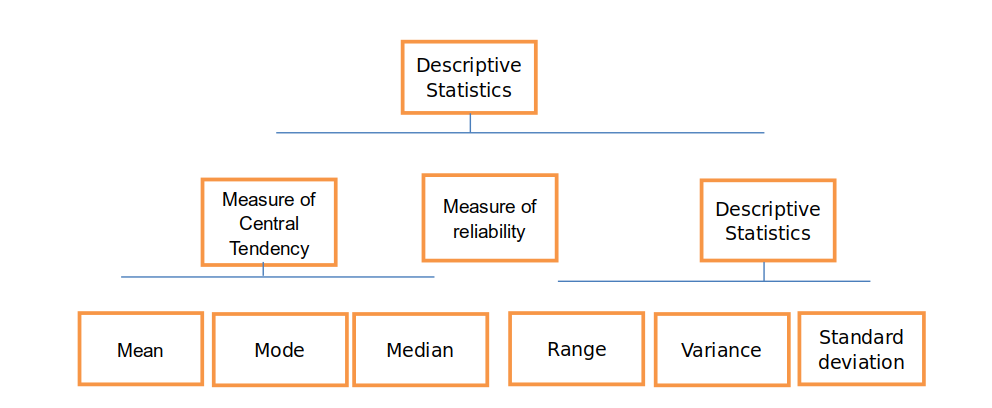
\includegraphics[width=0.85\textwidth]{Fig1.png}
 \caption{An example of a graphic organizer filled by a student teacher.}
 \label{fig01}
 \source{Own elaboration.}
\end{figure}

Large and small group instruction, as well as cooperative learning, were utilized in the classroom lesson. As \textcite{tomasello_natural_2014} argues, verbal thinking emerges from cultural society activity through shared intentionality and social collaboration \cite{negueruelaazarola_internalization_2013}. The primary goals in the classroom should be to promote strategic social interaction \cite{di_pietro_strategic_1987} and meaningful, significant interaction in which students construct new knowledge on their own. Engaging students in social interaction is an important part of transformative pedagogy for EFL classrooms. From this current perspective, language instruction is fundamentally about personal transformation (defined as the outcome of conceptual development) for both learners and teachers. Theory and practice are inextricably linked through a dialectical relationship, with theory guiding practice and practice feeding theory, allowing for a bidirectional shift change in both \cite{lantolf_sociocultural_2014}.

\section{Conclusion}\label{sec-secoes}
The findings indicate three key pedagogical implications. Firstly, the SIOP model can be integrated into a university course that emphasizes (1) lesson preparation, (2) building background, (3) comprehensible input (appropriation), (4) strategies, (5) interaction, (6) practice/application, (7) lesson delivery, (8) review and assessment. Second, the findings indicate that the implementation of the SIOP model engages students in disciplinary vocabulary learning while also making the content concept more accessible to the students in the class. In addition, the SIOP model encourages dynamic classroom activities and develops students' language skills (reading, writing, and oral proficiency) because students have several opportunities to talk to each other and use sentences like "In my view..." or "Based on the results, we come to...". Finally, the SIOP model can help students develop their lexico-grammatical competence and academic language autonomy. The current study demonstrates the application of the SIOP model in a content curriculum program. The author think that more research will show how the SIOP model is used in content curriculum programs, especially when students are learning English in class for a specific purpose in various Asian nations where English is not the native language Pedagogically, there is an urgent need for quantitative research involving English as a foreign language teachers to use SIOP in the English Language Education Program in order to engage students in learning QR in the ELT research to apply learning content and language in order to practice the academic language as it is used in disciplinary or specific topic areas.

\printbibliography\label{sec-bib}
% if the text is not in Portuguese, it might be necessary to use the code below instead to print the correct ABNT abbreviations [s.n.], [s.l.]
%\begin{portuguese}
%\printbibliography[title={Bibliography}]
%\end{portuguese}


\appendix
\section{SIOP lesson plan template}\label{appendix} 

\begin{table}[htbp]
\begin{threeparttable}
\caption{SIOP lesson plan template.}
\label{tab11}
\centering
\begin{tabular}{p{\textwidth}}
\toprule
SIOP lesson plan template   \\
\midrule
Topic: 
\vspace{7ex} \\
\midrule
Content Objectives: 
\vspace{7ex} \\
\midrule
Language Objectives: 
\vspace{7ex} \\
\midrule
Key Concepts and Vocabulary: 
\vspace{7ex} \\
\midrule
Supplementary Materials: 
\vspace{7ex} \\
\midrule
Preparation: 
\vspace{7ex} \\
\midrule
Motivation:
\vspace{7ex} \\
\midrule
Presentation: 
\vspace{7ex} \\
\midrule
Practice/Application: 
\vspace{7ex} \\
\midrule
Review/Assessment: 
\vspace{7ex} \\
\midrule
Extension Activities:
\vspace{7ex} \\
\bottomrule
\end{tabular}
\source{Own elaboration}
\end{threeparttable}
\end{table}


\end{document}

